
\section{Statement of Work (SOW)}
The project's aim is to develop a minaturized high-sensitivity, low-noise magnetic gradiometer. Our approach is to mimic the mechanism found in magnetosomes, the specialized cells four from bacteria to higher vertebrates such as fish and birds (see \ref{sec:inno}). This is comprised of four main tasks: modeling and simulation, microfabrication process design, circuit design, and device manufacture and testing. Each Phase (I,II,III) will include these four tasks.

\subsection{Phase I}

AMBIIENT Phase 1 will demonstrate sensor functionality and performance in a laboratory
setting meeting the performance metrics as indicated in Table \ref{table:obj}. 

\subsubsection{Modeling and simulation}\label{sec:p1:em}
\begin{itemize}
\item The objective in this phase is to simulate the MEMS device, taking into account geometry, material properties, and multiphysics interactions, in order to determine the range of acceptable design options. In addition, scaling laws will be derived, such that a scale model of the sensor could be fabricated from COTS components.
\item Our approach here is to initially specify geometry and physical properties by hand calculation, the investigae more deeply in a finite-element multiphysics solver.
\item This task will be accomplished at UF by Joaquin Casanova.
\item Completion of this task is specified by successful simulation of the MEMS device that meets the physical requirements specified in the BAA.
\item Deliverables include successful simulation results and design parameters.
\item No government equipment is required.
\item To reduce risk of later failure due to non-manufacturability, this task will be accomplished within fabrication constraints specified by the MEMS team at UF. This ensures the design is physically realizable. In parallel, other sensing modalities could be explored in the case that the MEMS cantilever is not practical.
\end{itemize}
\subsubsection{Microfabrication}\label{sec:p1:mf}
\begin{itemize}
\item The objective in this phase is to develop a microfabrication strategy (materials, deposition, patterning) that can meet the requirements found from simulation.
\item Our approach here is to find a range of dimensional constraints and material types that could be physically realizable, and use those options to guide simulation and design of a sensor.
\item This task will be accomplished at UF by Dr. YK Yoon.
\item Completion of this task is successful specification of a microfabrication plan for the sensor described by the simulation results.
\item Deliverables include successful microfabrication plan.
\item No government equipment is required.
\item To reduce risk of later failure due to non-manufacturability, this task will be accomplished with parallel investigating of alternative MEMS sensing modalities.
\end{itemize}
\subsubsection{Circuit design}\label{sec:p1:cir}
\begin{itemize}
\item The objective in this phase is to develop a circuit which amplifies and digitizes the the voltage produced by the MEMS elements. Ina ddition to a COTS circuit, we will simultaneously begin investigation of an IC that can be used in later phases.
\item Our approach here is to ...
\item This task will be accomplished at TTU by Dr. Changzi Li.
\item Completion of this task is specified by successful design of a circuit capable of amplifying and digitizing MEMS output voltage with input-referred voltage noise low enough to meet the overall sensitivity requirement.
\item Deliverables include successful design and prototype of the circuit, usable with the fabricated MEMS sensor head, using COTS components.
\item No government equipment is required.
\item To reduce risk of later failure due to excessive noise, this task will investigate only specifically low-noise designs.
\end{itemize}
\subsubsection{Manufacture and testing}
\begin{itemize}
\item The objective in this phase is to construct the MEMS design using microfabrication processes and design developed in \ref{sec:p1:em},\ref{sec:p1:mf}, which includes pads for connection to circuitry.
\item Our approach here is to 
\item This task will be accomplished at UF by Dr. Yoon and Dr. Joaquin Casanova.
\item Completion of this task is specified by successful construction and testing of a sensor head, which satisfies Table \ref{table:obj}, using the circuitry developed in \ref{sec:p1:cir}.
\item Deliverables include successful prototype of the sensor and sensor electronics.
\item No government equipment is required.
\item To reduce risk of failure, fabrication will begin early in Phase 1, enabling us to revise our design to reduce manufacturing defects orenhance sensivity. 
\end{itemize}
\subsection{Phase II}
  
AMBIIENT Phase 2 will develop and demonstrate an integrated sensor head meeting the
performance and SWaP metrics of Table \ref{table:obj}, and including all vacuum, photonic, and thermal
control components.


IC design? Size?
\subsubsection{Modeling and simulation}
\subsubsection{Microfabrication}
\subsubsection{Circuit design}
\subsubsection{Manufacture and testing}
\subsection{Phase III}
AMBIIENT Phase 3 will demonstrate a fully integrated gradiometer comprising all control
electronics, power conditioning, and packaging, meeting all performance metrics of Table  \ref{table:obj}


ADC? Size?
\subsubsection{Modeling and simulation}
\subsubsection{Microfabrication}
\subsubsection{Circuit design}
\subsubsection{Manufacture and testing}

\section{Innovative Claims}\label{sec:inno}

Our approach is to design a sensor based on a magnetoreceptive mechanism used in nature - magnetite crystals torqued by external magnetic fields open ion channels in the cell wall. To mimic this, we propose a microfabricated MEMS sensor, with a layer of magnetic material on top of piezo electric cantilevers. When forced with an exernal field, torque induced on the magnet create stress in the piezo, and thus a voltage is produced. There are three advantages to this approach. First, microfabrication allows for a small size. Second, by orienting individual sensing elements in anti-series order, the output is natively a gradiometer. Third, by selecting the resonant frequency of the cantilever carefully, we can create a gradiometer which outputs a spectrogram directly. Though fluxgates can be microfabricated and function as gradiometers, they suffer a size/sensitivity tradeoff. Microfabricated atmonic magnetometers are sensitive but don't function natively as gradiometers. Other micro-scale magnetometers, namely Lorentz-type, which operate on a similar mechanism, are not yet sensitive enough and haven't been used as frequency-domain gradiometers, as in the proposed design.

\section{Detailed Technical Approach}

\begin{figure}[h]
  \centering
  \begin{subfigure}
    \centering
    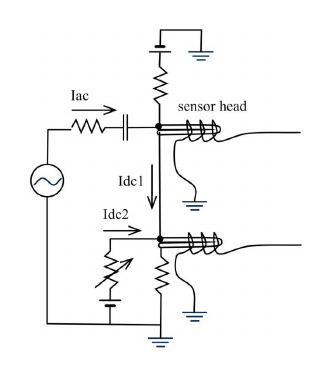
\includegraphics[width=0.5\textwidth]{fmofg}
  \end{subfigure}
  \begin{subfigure}
    \centering
    
\includegraphics[width=0.5\textwidth]{fmofg2}
  \end{subfigure}
\caption{Fundamental-mode orthogonal fluxgate gradiometer \cite{sasada2014fundamental}.}
\label{fig:fmofg}
\end{figure}

\begin{figure}[h]
\centering
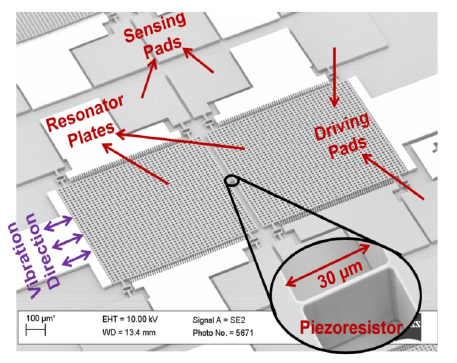
\includegraphics[width=0.5\textwidth]{lorenz2}
\caption{Lorenz-type magnetometer \cite{kumar2015ultra}.}
\label{fig:lorenz}
\end{figure}

Magnetometers serve an important role in investigating biologically generated electromagnetic fields, such as those created by neuronal currents, or geological magnetic fields. Typically, magnetometers are unable to achieve high sensitivity in an ambient, unshielded environment - getting to femtotesla level sensitivity requires magnetic shield and cryogenic sensors, such as SQUID \cite{lenz2006magnetic}. The novel spin relaxation free magnetometer has been minaturized and achieves less than 10 fT/$\sqrt{Hz}$, but still requires shielding and lacks directional sensitivity \cite{shah2013compact}. Fluxgates (Figure \ref{fig:fmofg}) have achieved pT level resolution at small size, but this is insufficient for biomagnetic field measurement \cite{sasada2002orthogonal,uchiyama2014highly,sasada2014fundamental} 

Lorenz-type magnetometers (which translate magnetic fields into mechanical actuation of a magnet or current carrying wire) have been built in MEMS substrates (Figure \ref{fig:lorenz}), but are as yet insufficiently sensitive and require shielding \cite{sinha201627,kyynarainen20083d,kumar2015ultra,thompson2009parametrically}

\begin{figure}
\centering
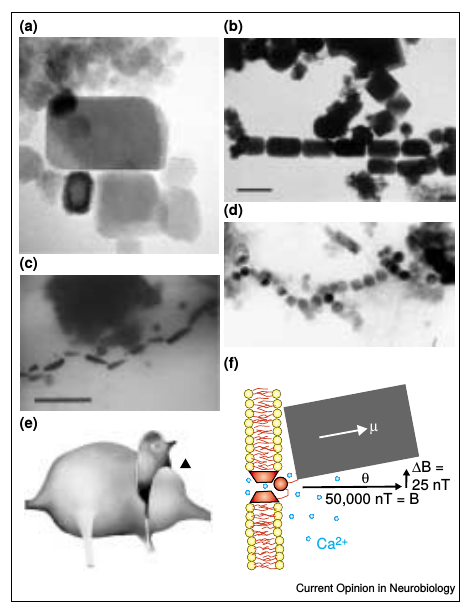
\includegraphics[width=0.5\textwidth]{kirsh2001}
\caption{Magnetosomal mechanism \cite{kirschvink2001magnetite}.}
\label{fig:magnetosome}
\end{figure}

In nature, many organisms have a sense of magnetoreception used for navigation, from magnetotactic bacteria to birds. Two mechanisms have been proposed: a spin-selective (and thus field-sensitive) chemical reaction rate, or magnetite crystals which are actuated by external fields and activate ion channels in the cell membrane (Figure \ref{fig:magnetosome})\cite{johnsen2005physics,dodson2013radical,kirschvink2001magnetite}. Measurements of these magnetosomes show a magnetic dipole moment of up to 100fA/m$^2$ \cite{hanzlik2002pulsed,eder2012magnetic}.

Our approach is to mimic the approach found in magnetosomes, with some key modifications so that is frequency-selective and functions inherently as a gradiometer and thus does not require shielding. The closest biomimetic sensor is a flow sensor which uses ferromagnetic cilia to detect microfluidic flow rates \cite{alfadhel2014magnetic}.

\begin{figure}[h]
\centering
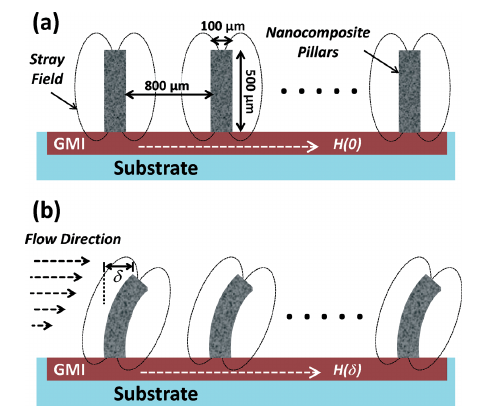
\includegraphics[width=0.5\textwidth]{cilia}
\caption{Magnetic cilia flow sensor \cite{alfadhel2014magnetic}.}
\label{fig:cilia}
\end{figure}

To acomplish this, we propose layering a permanent magnetic layer on top of piezoelectric cantilevers. The moment $M$ induced on the magnetic layer with moment $\vec{\mu}$ and field $\vec{B}$ is:


$$  M=\vec{\mu} \times \vec{B} $$

Interpreted as a point load ($M/L$) at the cantilever tip, this moment causes a stress distribution on a cantilever of length L, thickness t, second moment I, piezoelectric constant $g_{31}$, and modulus E, at point x, of

$$ \sigma=\frac{Mt(L-x)}{2LI} $$

and $n$ in series generates a voltage

$$ V=\int_0^L\frac{Mt(L-x)}{2LI}g_{31}ndx $$

 Two features are possible from the cantilever design: frequency selection and gradiometery. As in \cite{shen2008design}, a cantilever has a resonant frequency, which can be modified through geometrical parameters. Peak response will be achieved at this frequency. By selecting many cantilevers of different dimensions, each corresponding to a separate output, the magnetometer output is a spectrometer. Many cantilevers at the same resonance in series generate a largeer voltage; in anti-series, the difference is taken, thus functioning as a gradiometer with very high spatial resolution (Figure \ref{fig:diagram}). 

 Even though biological magnetoreception is limited to nT sensitivity, our design will allow us to surpass this. First, by careful selection of materials (such as Co-Pt or rare-earth magnets) \cite{coey2010magnetism, arnold2009permanent} we can have much higher magnetic dipole moment, and thus higher moment. Second, by careful selection of geometery, we can employ parametric resonance \cite{van2006resonant}. Finally, using two banks of cantilevers in series in anti-series, we both boost the voltage and create a high resolution gradiometer.

 The noise floor of magnetic materials is governed by Barkhausen noise - the random flipping of magnetic domains \cite{butta2012sources}; this noise is characterized as a flux noise level. The flux noise can be converted into a magnetic moment noise, and thus moment noise. Piezo noise floor is largely a function of piezo losses \cite{levinzon2004fundamental}. Additionally, there is the input-referred noise of any amplifier. With conservative estimates for all of these, and two anti-series banks of 30 cantilevers each with dimensions 400x40x3 $\mu$m, the sensitivity level is less than 10 fT/cm/$\sqrt{Hz}$.

\begin{figure}
\centering
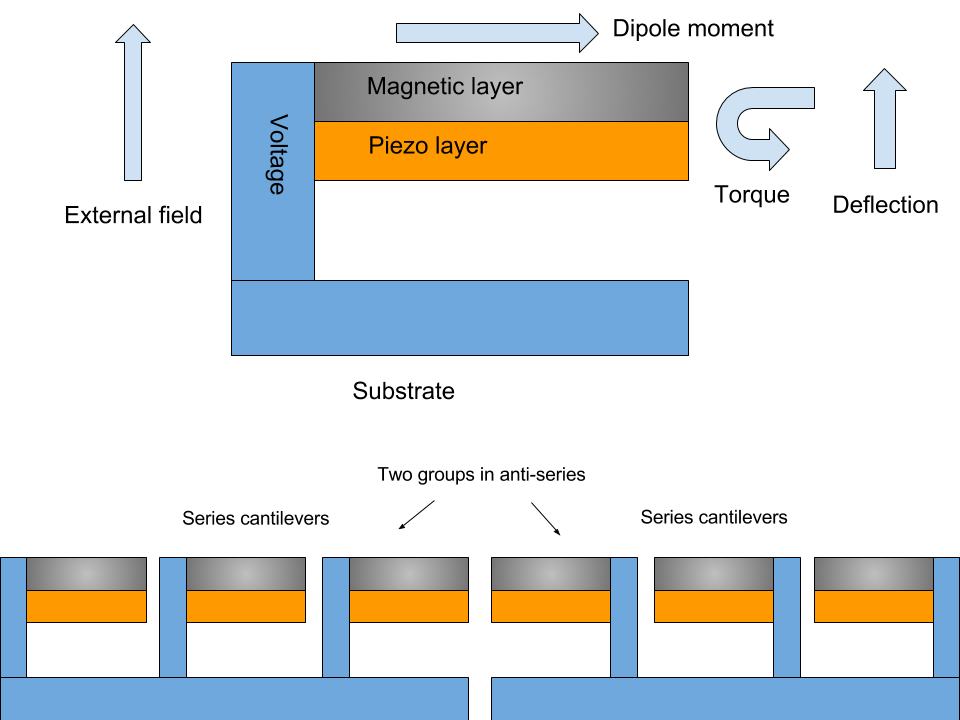
\includegraphics[width=0.75\textwidth]{biomag}
\caption{Diagram of proposed design.}
\label{fig:diagram}
\end{figure}

MEMS fabrication processes are capable of constructing the above-described sensor. This consists of two main fabrication tasks: piezo cantilever construction, and magnetic material integration. The process described in \cite{shen2008design} can be used for our task, with an additional step to apply the magnetic layer. PZT has a high voltage coefficient and is highly suitable for the piezo elements \cite{tadigadapa2009piezoelectric} and can be deposited with pulsed laser deposition or solution-based deposition and patterned with chemical etching or ion etching. Rare-earth magnetic materials, such as alloys of Sm-Co, offer high magnetic energy product at room temperature and can be integrated into MEMS using sputtering or pulsed laser deposition \cite{arnold2009permanent}. However, patterning of these materials is slow, using wet etching or ion-beam milling. A likely strategy will be to use a sacrificial polymer pattern, depositing electrodes, piezo, then magnet layers, and then etching the sacrificial layers. 

There are two possible circuit approaches we can consider for this cantilever approach. On one hand, very many small cantilevers, arranged in series in groups; or multiple, larger cantilevers. In the former case, we would individually address the sensor banks, effectively fitting multiple sensors on the same substrate, allowing differential or common-mode measurements. Many, smaller cantilevers would require a voltage amplifier; additionally, smaller cantilevers have higher resonant frequency, so in order to operate near resonance for maximum sensitivity they would need to be externally driven near resonance, and the signal would be demodulated to get measurements of the baseband signals. In the second approach, a few, larger cantilevers would have lower resonant frequencies and could directly sense at baseband. Their larger area produces a larger charge, so a charge amplifier would be more suitable. Ultimately, the number and size of cantilevers, and the circuit approach, is a tradeoff between the complexity of the interconnects, resonance of the structures, and the number of cantilevers which fit in the target volume.

\begin{table}[h!]
\centering
  \begin{tabular}{|c||c|c|c|}
    \hline
    Metric & Phase 1 & Phase 2 & Phase 3 \\
    \hline
    \hline
    Power consumption & 150 mW & 50 mW & 100 mW \\
    \hline
    Sensor Volume & 3x3x10 cm & 1x1x7 cm & 1x1x7 cm \\
    \hline
    Control Electronics Volume  & N/A & N/A & < 20cm$^2$ \\
    \hline
    Ambient Magnetic Field & $\pm$ 100 $\mu$T & $\pm$ 100 $\mu$T & $\pm$ 100 $\mu$T \\
    \hline
    Ambient Operating Temperature & N/A & 0$^{\circ}$ C to 50$^{\circ}$ C & 0$^{\circ}$ C to 50$^{\circ}$ C \\
    \hline
    Gradient Full-scale Range & 1 nT/cm & 1 nT/cm & 1 nT/cm \\
    \hline
    Gradient Sensitivity & 10 fT/cm/$\sqrt{Hz}$ & 3 fT/cm/$\sqrt{Hz}$  & 1 fT/cm/$\sqrt{Hz}$ \\
    \hline
    Gradient Accuracy & 100 fT/cm & 30 fT/cm & 10 fT/cm \\
    \hline
    Total Field Range & 100 $\mu$T & 100 $\mu$T & 100 $\mu$T \\
    \hline
    Total Field Sensitivity & 100 pT/$\sqrt{Hz}$ & 30 pT/$\sqrt{Hz}$  &  10 pT/$\sqrt{Hz}$ \\
    \hline
    Total Field Accuracy & 1 nT & 500 pT & 100 pT \\
    \hline
    Data Rate & 100/s & 200/s & 500/s \\
    \hline
    3 dB Bandwidth & 200 Hz & 400 Hz & 1000 Hz\\
    \hline
  \end{tabular}
\caption{Design objectives, by phase.}
\label{table:obj}
\end{table}

\begin{table}[h!]
\centering
  \begin{tabular}{|c||c|c|}
    \hline
    Phase & Milestone & Date\\
    \hline
    \hline
    1 & Cantilever simulation and design & \\
    \hline
    1 & Fabrication plan & \\
    \hline
    1 & Circuit design & \\
    \hline
    1 & Scale model design and testing & \\
    \hline
    \hline
    2 & Cantilever simulation and design & \\
    \hline
    2 & Fabrication plan & \\
    \hline
    2 & Circuit design & \\
    \hline
    2 & MEMS fabrication and testing & \\
    \hline
    \hline
    3 & Cantilever simulation and design & \\
    \hline
    3 & Fabrication plan & \\
    \hline
    3 & Circuit design & \\
    \hline
    3 & MEMS fabrication and testing & \\
    \hline
  \end{tabular}
\caption{Milestones schedule}
\label{table:sched}
\end{table}

\section{Risk Analysis and Mitigation Plan}

\begin{table}[h!]
\centering
\begin{tabularx}{.85\textwidth}{|X||c|c|X|}
    \hline
    Risk & Probability & Impact & Plan\\
    \hline
    \hline
    Insufficient sensitivity in simulation & 3 & 10 & Optimize design architecture. \\
    \hline
    Best available MEMS processes infeasible & 4 & 10 & Begin design process within constraints of available processes. \\
    \hline
    Interconnects infeasible & 3 & 5 & Operate fewer, larger cantilevers \\
    \hline
    Viscous damping hurts sensitivity & 3 & 5 & Operate in vacuum packaging \\
    \hline
    Resonance frequency infeasibly high & 3  & 5 & Operate fewer, larger cantilevers \\
    \hline
    Fabrication unreliable/mismatch & 3 & 5 & Begin fabrication early, so process can be adjusted; dynamic element matching. \\
    \hline
    Fabrication time/window exceeds deadlines & 3 & 5 & Fabricate COTS scale model instead. \\
    \hline
    Circuit/sensor sensitive to mechanical vibration & 5 & 8 & Use additional sensors without magnetic layer to independently measure mechanical vibrations. \\
    \hline
    Circuit/sensor fails final tests & 3 & 9 & Identify points of failure for next design. \\
    \hline
\end{tabularx}
\caption{Risk matrix}
\label{table:risk}
\end{table}

There are several risks and challenges associated with this design. Most can be addressed simply by doing careful analysis of the problem within the range of constraints on materials and processes. Others (the density of interconnects, or resonant frequency, is too high) can be address by reducing the number of elements and increasing their size. Damping do to the viscosity of air could hurt sensitivity could be addressed by vacuum packaging the sensor head. Manufacturing mismatch of the sensing elements can be effectively removed by dynamic element matching, where the transducers are switched electronically to average out fabrication differences.

\section{Schedule and Milestones}
Include a high-level Gantt chart outlining major technical tasks and measureable milestones
by phase. At a minimum, the schedule should include each SOW task of Volume 1, Section
II.A. Where risk reduction tasks are proposed, the schedule should include a milestone for
assessment and removal of redundant tasks.

\section{Test Plan}

To test, in Phase 1, the sensor will first be connected to the circuitry and powered to established basic functionality.  Prior to testing, noise from the Helmholtz coils, power supplies, and any other necessary signal generation sources will be characterized. Further, the sensor will be placed in a pair of Helmholtz coils driven with precision current sources, inside magnetic shield, so we can gauge accuracy and sensitivity in a controlled environment. Field gradient, intensity, and frequency will be swept over the range specified in \ref{table:obj}. Finally, the same test will be repeated in an unshielded environment. In each case, we will monitor power consumption, signal output, and mesure sensor and sensor control electronics volume. Subsequent phases will follow a similar testing protocol, except using specifications for those phases. Additionally, in Phases 2 and 3, where an IC will be developed and integrated with the sensor head, the IC will be tested independently to verify basic input/output functionality before slicing and bonding to the MEMS substrate.

\section{Results and Technology Transfer}
Description of the results, products, transferable technology, and expected technology
transfer. This should also address mitigation of life-cycle and sustainment risks associated
with transitioning intellectual property for U.S. military applications, if applicable. See also
Section IV.B.10, “Intellectual Property.”

\section{Ongoing Research}
Presently, Drs. Lin, Li, and Casanova are presently involved (until 6/2017) in a DARPA project for detection and inversion of MEG/EEG signals. They have worked on all phases, from sensor design to circuit design to inversion algorithm. Additionally, Drs. Lin and Li have worked exensively on vital signs radar, and Dr. Casanova has worked on electromagnetic sensors for agriculture and analytical chemistry. Dr. Yoon has conducted research in MEMS systems of all types, including piezoelectronics and magnetics. Presently his work ...

\section{Facilities}

Facilities at UF for sensor development and testing include magnetic shielding, circuit testing instrumentation (power supplies, oscillopes, function generators, VNA). For fabrication, the Nanoscale Research Facility at UF includes equipment for a variety of processes: plasma, vapor, and sputtering deposition, annealing, wafer bonding, wire bonding, UV and e-beam lithography, reverse ion etching, and wet etching.

TTU?

\section{Teaming/Proposer Accomplishments}

\begin{description}
\item[UF] The UF team incluldes the following personnel:
  \begin{description}
  \item[Jenshan Lin] will be project lead, and supervise work on the AMBIIENT project. His time commitment is 0\%. He received the B.S. degree in Electrophysics from National Chiao Tung University (NCTU), Hsinchu, Taiwan, R.O.C., in 1987, and the M.S. and Ph.D. degrees in Electrical Engineering from the University of California at Los Angeles (UCLA), in 1991 and 1994, respectively. His current research interests include sensors and biomedical applications of microwave and millimeter-wave technologies, wireless energy transfer and conversion, RF system-on-chip integration, and integrated antennas. Dr. Lin has authored or co-authored over 250 technical publications in refereed journals and conference proceedings. He holds 15 patents and has several other patent applications. Since joining University of Florida, he has graduated 22 PhD students. 
  \item[Joaquin Casanova] will conduct electromagnetic simulation and design of the MEMS sensor, and work with Dr. Yoon on process/material selection, and Dr. Li on requirements for the interface and control circuits. His commitment is 50\%. He received a B.S. and M.E. in Agricultural and Biological engineering in 2006 and 2007 from UF, and PhD in Electrical Engineering in 2010 from UF. His work has primarily focused on sensors and electromagnetic design, including wireless power, microwave remote sensing, agricultural sensors, analytical chemistry equipment design, and low-field magnetic sensing. He is currently a Research Assistant Professor in UF's Department of Electrical and Computer Engineering. 
  \item[YK Yoon] will guide selection of a microfabrication process and fabrication of the sensor. His commitment is 10\%. He received his BS and MS degrees in electrical engineering from Seoul National University in Korea. He also earned an MSEE degree from the New Jersey Institute of Technology, Newark, NJ in 1999 and the Ph.D. degree in electrical and computer engineering from the Georgia Institute of Technology, Atlanta, GA in 2004. He is currently an Associate Professor in the Department of Electrical and Computer Engineering at the University of Florida, Gainesville, FL. His current research interests include three dimensional (3-D) micromachining and nano fabrication; design and implementation of metamaterial for radio frequency (RF) and microwave applications; micromachined millimeter wave and terahertz antennas and waveguides; bio/microfluidic systems for the lab-on-a-chip applications; wireless telemetry systems for biomedical applications; and ferroelectric material development for high density memory devices and/or tunable RF devices.
  \end{description} 
\item[TTU] The TTU team includes:
  \begin{description}
  \item[Changzhi Li] will design the electronics for amplifying and digitizing the signals from the sensor head, working with Dr. Casanova to determine ciruit requirements. His time commitment is 10\%. He received the B.S. degree in electrical engineering from Zhejiang University, China, in 2004 and the Ph.D. degree in electrical engineering from the University of Florida, Gainesville, FL, in 2009.In the summers of 2007 and 2008, he worked at Alereon Inc., Austin, TX, on ultrawideband (UWB) transceiver. In the summer of 2009, he worked at Coherent Logix Inc., Austin, TX, on software-defined radio. His research interests include analog circuits, microwave circuits, and biomedical applications of microwave/RF.
  \end{description}
\end{description}
